\chapter{Validazione (parte 1): model selection e model
assessment}\label{ch-09}

La validazione è stata introdotta in
\href{04\%20-\%20Generalizzazione\%20e\%20validazione\%20(introduzione)}{04
- Generalizzazione e validazione (introduzione)}; queste lezioni la
approfondiscono, perché è indispensabile per il progetto e per ogni
applicazione seria del ML. Si ribadiscono i due obiettivi (model
selection e model assessment), si vede un controesempio che mostra
quanto è facile ottenere stime sbagliate, si introducono la \textbf{grid
search} e la \textbf{K-fold cross-validation}, e si discutono
campionamento, pochi dati e misure d'errore.

\section{Premessa: bias e varianza}\label{premessa-bias-e-varianza}

La decomposizione \textbf{bias-varianza} (che avrà una lezione dedicata)
è un quadro utile per capire perché stimare le prestazioni di un modello
è difficile: mostra il ruolo delle diverse \textbf{realizzazioni del
training set} e, ancora una volta, il compromesso tra capacità di
adattamento (bias) e flessibilità del modello (varianza).

\begin{figure}[htbp]
\centering
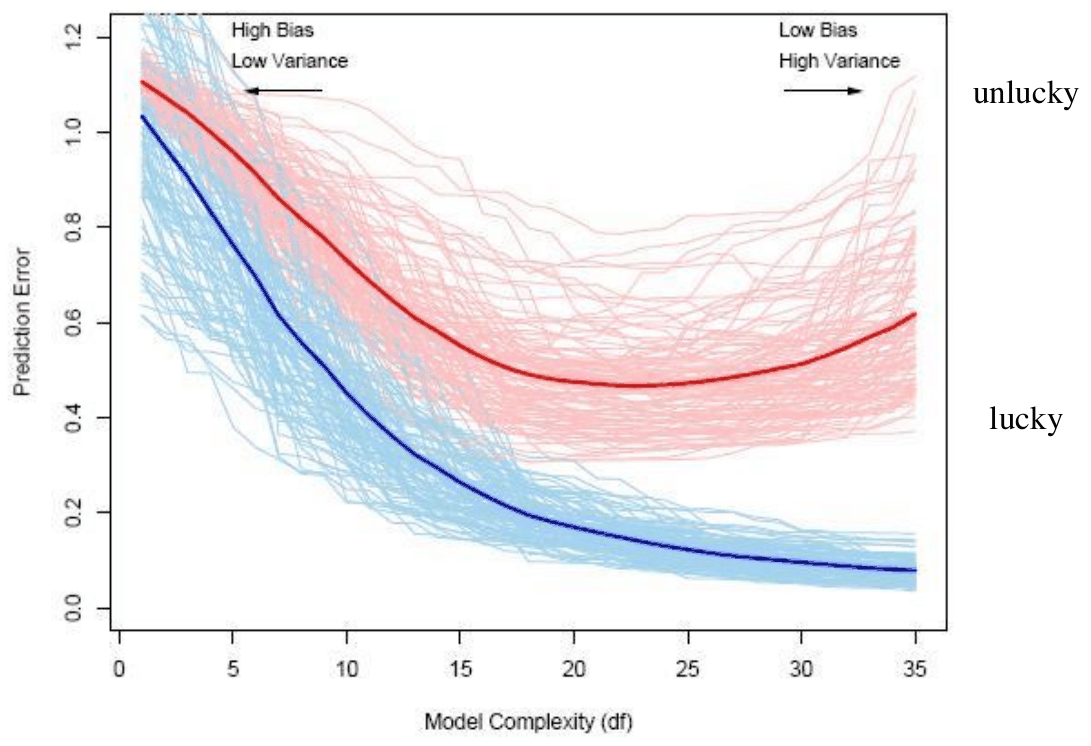
\includegraphics[width=0.71\linewidth,height=0.42\textheight,keepaspectratio]{images/09-val1_bias-varianza.png}
\caption{Errore di training (azzurro) e di test (rosso) su 100 training set
diversi al crescere della complessità (Hastie et al., Fig. 7.1). Con un
modello complesso il bias è basso ma la varianza alta: a seconda del
campione si può essere ``fortunati'' o ``sfortunati''.}
\end{figure}

La figura mostra un fatto importante: a parità di complessità, l'errore
di test varia molto tra un training set e l'altro, soprattutto per
modelli complessi. Una singola misura può essere fortunata o sfortunata.

\section{Motivazioni}\label{motivazioni}

Cerchiamo la soluzione con il minimo errore di predizione (di test),
bilanciando \textbf{adattamento ai dati di training} e
\textbf{complessità del modello}. L'errore di training \textbf{non è una
buona stima} dell'errore di test: all'inizio c'è troppo bias
(underfitting, errore di training alto), poi troppa varianza (errore di
training basso ma overfitting).

Supponendo di avere un iperparametro \(\theta\) (implicito o esplicito)
che regola la complessità del modello, vogliamo il valore di \(\theta\)
che minimizza l'errore di test. Servono quindi metodi per
\textbf{stimare l'errore atteso} di un modello (o di ciascun modello di
una classe, o di un insieme di modelli).

\subsection{Come stimare}\label{come-stimare}

\begin{itemize}
\tightlist
\item
  \textbf{Analiticamente}: criteri AIC e BIC (\emph{Akaike/Bayesian
  Information Criterion}, limitati a modelli lineari nei parametri), MDL
  (\emph{Minimum Description Length}), \textbf{SRM} (\emph{Structural
  Risk Minimization}) con la VC-dimension (vedi la lezione sulla SLT).
\item
  \textbf{Empiricamente}, sui dati, tramite \textbf{ricampionamento}
  (stima diretta dell'errore fuori campione): \textbf{cross-validation}
  (hold-out, K-fold, \ldots) e \textbf{bootstrap}.
\end{itemize}

\section{I due obiettivi della
validazione}\label{i-due-obiettivi-della-validazione}

\begin{boxwarning}{La slide più importante del corso}

Dopo aver addestrato i modelli sul training set:

\begin{itemize}
\tightlist
\item
  \textbf{Model selection}: stimare le prestazioni (errore di
  generalizzazione) di diversi modelli per \textbf{scegliere il
  migliore}. Include la ricerca dei migliori \textbf{iperparametri}
  (grado del polinomio, numero di unità di una rete, \(\lambda\),
  \(\eta\), \ldots). \emph{Restituisce un modello.}
\item
  \textbf{Model assessment}: scelto il modello finale (o una classe di
  modelli), \textbf{stimarne l'errore di predizione} (rischio) su dati
  di test nuovi, come misura della qualità del modello scelto.
  \emph{Restituisce una stima.}
\end{itemize}

\textbf{Regola d'oro}: tenere separati gli obiettivi e usare
\textbf{insiemi di dati separati} in ogni fase.

\end{boxwarning}

\subsection{Hold-out}\label{hold-out}

Se i dati sono sufficienti si divide il dataset in tre insiemi
\textbf{disgiunti}, ad esempio 50\% TR, 25\% VL, 25\% TS:

\begin{itemize}
\tightlist
\item
  \textbf{TR} (\emph{training set}): per adattare il modello, cioè
  minimizzare \(R_{emp}\) della SLT {[}\textbf{training}{]};
\item
  \textbf{VL} (\emph{validation} o \emph{selection set}): per scegliere
  il modello migliore tra modelli e configurazioni di iperparametri
  diversi {[}\textbf{model selection}{]};
\item
  \textbf{TS} (\emph{test set}): per stimare l'errore di
  generalizzazione del modello finale, cioè stimare \(R\) della SLT
  {[}\textbf{model assessment}{]}.
\end{itemize}

TR e VL insieme formano il \textbf{development/design set}, usato per
costruire il modello finale.

\begin{boxnote}{Due precisazioni}

\begin{enumerate}
\def\labelenumi{\arabic{enumi}.}
\tightlist
\item
  La stima fatta sul VL serve \textbf{solo} alla model selection: non è
  una buona stima per l'assessment.
\item
  I risultati sul TS \textbf{non} si possono usare per la model
  selection. Se lo si fa, quello non è più un test set: chiamiamolo
  validation set.
\end{enumerate}

\end{boxnote}

\subsection{Test o model selection?}\label{test-o-model-selection}

Cosa succede se il test set viene usato in un ciclo di progettazione
ripetuto (provo, guardo il test, cambio, riprovo)? Si sta facendo
\textbf{model selection}, non una valutazione affidabile, e non potremmo
farlo sugli esempi futuri. L'errore sul test così usato è una
\textbf{stima troppo ottimistica} dell'errore vero. È come un esercizio
d'esame di cui si sono viste le soluzioni: non è più un test! Da qui il
concetto di \textbf{blind test set} (test cieco), usato nelle
competizioni di ML.

\begin{figure}[htbp]
\centering
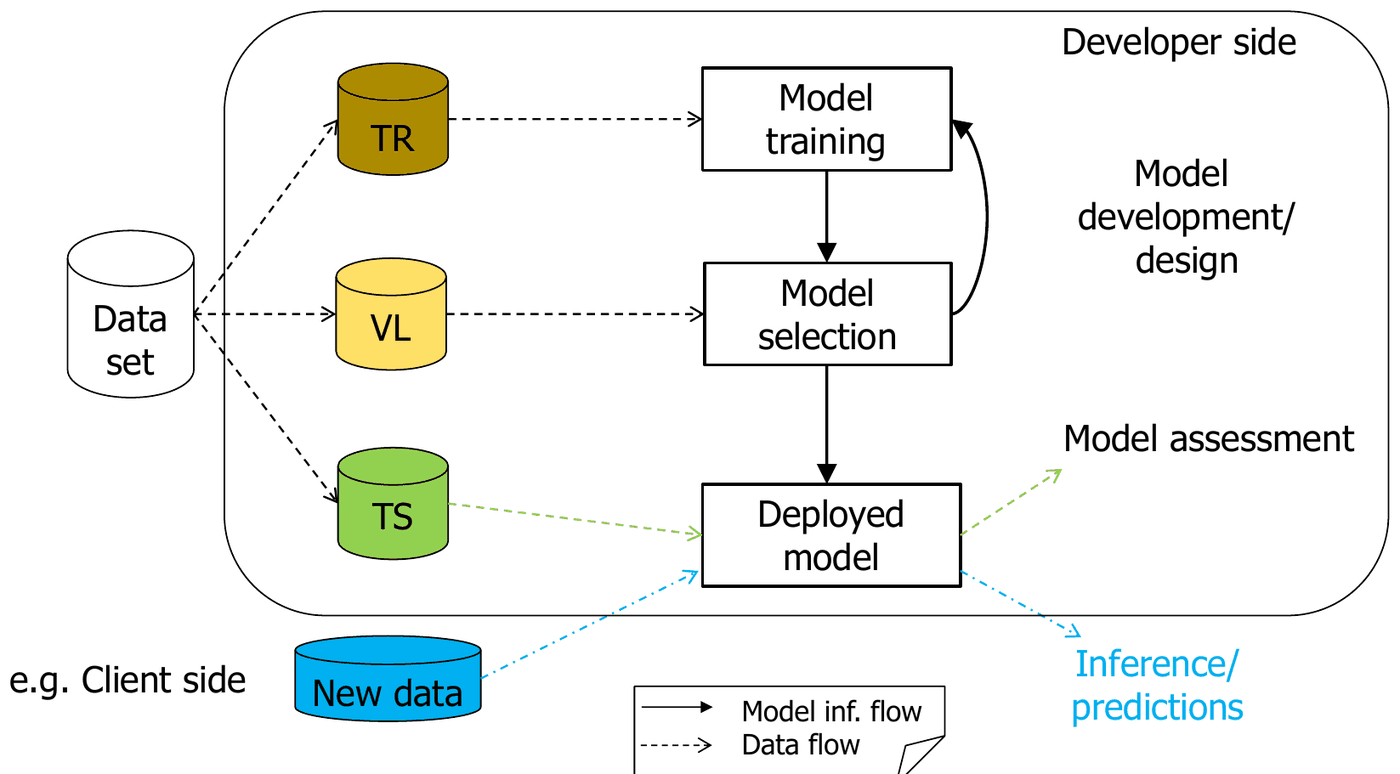
\includegraphics[width=0.80\linewidth,height=0.42\textheight,keepaspectratio]{images/04-l4_schema-tr-vl-ts.png}
\caption{Ruolo di TR, VL e TS (ripresa dalla lezione 4).}
\end{figure}

\section{Un controesempio istruttivo}\label{un-controesempio-istruttivo}

\begin{boxexample}{Il controesempio del target casuale}

\begin{itemize}
\tightlist
\item
  20--30 esempi, \textbf{1000 variabili di input} a valori casuali;
\item
  target \textbf{casuale} 0/1.
\end{itemize}

Si seleziona un modello che usa \textbf{una sola} variabile di input,
quella che per puro caso ``indovina'' il target al 99\% (o 100\%) su
qualsiasi successiva suddivisione in TR, VL e TS. Risultato perfetto?
Cosa c'è di sbagliato?

Il 99--100\% \textbf{non} è una buona stima dell'errore di test: quella
vera è il \textbf{50\%} (il target è casuale, nessun modello può fare
meglio di una moneta). Su un test set esterno davvero nuovo si
otterrebbe il 50\%.

\end{boxexample}

Gli errori sono due:

\begin{enumerate}
\def\labelenumi{\arabic{enumi}.}
\tightlist
\item
  la stima dell'errore su TR e VL \textbf{non è} una buona stima del
  rischio;
\item
  usare \textbf{l'intero dataset} per la selezione delle feature o del
  modello \textbf{pregiudica la stima} (stima distorta, detta
  \emph{subset selection bias}): il test set è stato usato
  \textbf{implicitamente} all'inizio, nella scelta della variabile. Il
  test set va separato \textbf{in anticipo}, prima di \textbf{qualsiasi}
  model selection, inclusa la \textbf{feature selection}.
\end{enumerate}

Con 1000 variabili casuali e soli 20 pattern, è quasi certo che una
variabile coincida per caso con il target sulla maggior parte dei
pattern. Poiché la scelta è fatta guardando \textbf{tutti} i dati,
quella variabile ``funziona'' su qualunque partizione successiva. Su
pattern davvero nuovi (TS1, TS2, TS3 nella tabella della slide) la
stessa variabile ha accuratezze del 100\%, 33\%, 66\%: puro caso.

\begin{boxwarning}{Attenzione}

Qui si discute la \textbf{correttezza della stima}, non la possibilità
di risolvere il task. La K-fold CV e altre tecniche \textbf{non}
risolvono il problema se la selezione è fatta prima della suddivisione
(anzi, possono confondere ancora di più).

\end{boxwarning}

\section{Grid search}\label{grid-search}

Gli \textbf{iperparametri} sono parametri non appresi direttamente
dall'algoritmo; si fissano cercando nello \textbf{spazio degli
iperparametri}, naturalmente tramite model selection su un validation
set.

La \textbf{grid search esaustiva} genera tutti i candidati da una
griglia di valori. Esempio banale con numero di unità e \(\lambda\):

{\def\LTcaptype{none} % do not increment counter
\begin{longtable}[]{@{}llll@{}}
\toprule\noalign{}
Unità ~\(\lambda\) & 0,1 & 0,01 & 0,001 \\
\midrule\noalign{}
\endhead
\bottomrule\noalign{}
\endlastfoot
1 unità & Res1 & Res4 & Res7 \\
10 unità & Res2 & Res5 & Res8 \\
100 unità & \textbf{Res3} & Res6 & Res9 \\
\end{longtable}
}

Se il migliore risultato (sul validation) è Res3, vince la
configurazione (100 unità, \(\lambda = 0{,}1\)). Va
\textbf{automatizzata}, ed è facile da \textbf{parallelizzare} (le prove
sono indipendenti).

Il costo può essere alto: è il prodotto cartesiano dei valori, cioè
\((\#\text{valori})^{\#\text{iperparametri}}\). Con 3 valori per 2
iperparametri sono \(3^2 = 9\) prove; con 5--6 iperparametri da 10
valori ciascuno diventa proibitivo. Per questo:

\begin{itemize}
\tightlist
\item
  si possono fissare alcuni iperparametri in una fase sperimentale
  preliminare, se si mostrano poco rilevanti (con cautela, vedi l'errore
  della selezione sequenziale nella parte 3);
\item
  si usano \textbf{due (o più) livelli di grid search annidate}: prima
  una ricerca \textbf{grossolana} su tutte le combinazioni (ad esempio
  con valori a crescita esponenziale) per trovare le regioni buone, poi
  ricerche \textbf{più fini} su intervalli sempre più piccoli, sempre
  considerando \textbf{tutti} gli iperparametri significativi insieme.
\end{itemize}

\subsection{Alternative alla grid
search}\label{alternative-alla-grid-search}

La grid search è molto utile per \textbf{osservare il comportamento} del
modello al variare degli iperparametri (fondamentale per capire), ma è
costosa e scala male con il numero di iperparametri. Alternative:

\begin{itemize}
\tightlist
\item
  \textbf{ricerca casuale} (Bergstra e Bengio, 2012): evita di
  ricampionare gli stessi valori di un iperparametro influente quando
  altri non lo sono, e permette di fissare il \textbf{budget} di prove
  indipendentemente dal numero di iperparametri;
\item
  ricerca \textbf{automatica}: approcci bayesiani, evolutivi, metodi di
  valutazione delle configurazioni (es. Hyperband).
\end{itemize}

Librerie come Keras Tuner e scikit-learn includono molte alternative
(verso l'\textbf{AutoML}), ma non vanno usate acriticamente: la grid
search insegna di più al primo approccio.

\begin{figure}[htbp]
\centering
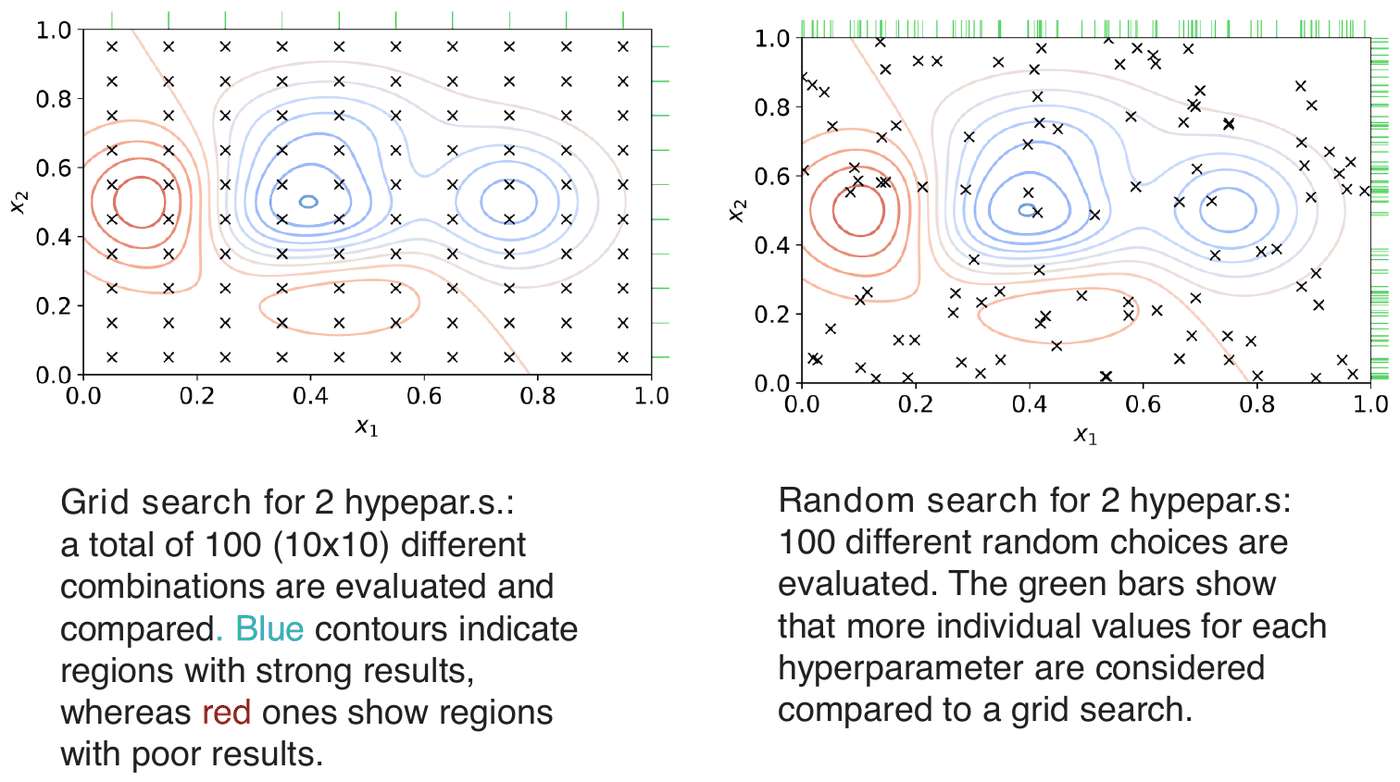
\includegraphics[width=0.91\linewidth,height=0.42\textheight,keepaspectratio]{images/09-val1_grid-random.png}
\caption{Grid search e random search con 100 prove ciascuna: la ricerca casuale
esplora molti più valori distinti di ciascun iperparametro (barre
verdi).}
\end{figure}

\begin{boxtip}{Perché la random search funziona}

Se uno solo dei due iperparametri conta davvero, la grid 10×10 ne prova
solo \textbf{10 valori distinti} (le altre 90 prove ripetono gli stessi
valori variando l'iperparametro inutile), mentre la ricerca casuale ne
prova \textbf{100}.

\end{boxtip}

\section{K-fold cross-validation}\label{k-fold-cross-validation}

\subsection{Quanti dati servono?}\label{quanti-dati-servono}

L'hold-out richiede dati sufficienti per tre partizioni significative.
Quanti? Dipende dalla complessità del modello e dal rapporto
segnale/rumore (ne servono pochi per un modello lineare su un task
linearmente separabile senza rumore). Come fare se i dati non bastano? E
come evitare di dipendere dalla \textbf{particolare partizione} scelta?
La K-fold CV aiuta.

\begin{boxnote}{Terminologia}

``Cross-validation'' indica sia un \textbf{approccio} alla model
selection basato sulla stima diretta dell'errore tramite ricampionamento
(anziché analitica), sia più specificamente le \textbf{implementazioni}
che stabiliscono come dividere i dati per la selezione e per la
valutazione (ad esempio la K-fold CV).

\end{boxnote}

\subsection{Richiamo}\label{richiamo}

Si divide \(D\) in \(K\) sottoinsiemi mutuamente esclusivi
\(D_1,\dots,D_K\); per ogni \(i\) si addestra su \(D \setminus D_i\) e
si valuta su \(D_i\). Così tutti i dati vengono usati sia per
l'addestramento sia per la valutazione. Non si ottiene un \textbf{unico
modello} (ce n'è uno per fold), ma si ottiene anche una
\textbf{varianza} (deviazione standard) sui fold per la propria classe
di modelli: il risultato si riporta come \textbf{media ± deviazione
standard}. Si può usare sia per il validation set sia per il test set.

Questioni: quanti fold (3, 5, 10, \ldots, \emph{leave-one-out})? Il
costo computazionale è spesso alto. Si può combinare con un validation
set o fare una doppia K-fold CV.

\subsection{Un esempio completo di selezione e
valutazione}\label{un-esempio-completo-di-selezione-e-valutazione}

\begin{enumerate}
\def\labelenumi{\arabic{enumi}.}
\tightlist
\item
  Dividere i dati in \textbf{TR} e \textbf{TS} (qui con hold-out, ma
  potrebbe essere una K-fold).
\item
  \textbf{Model selection}: usare una K-fold CV \textbf{interna} al TR
  (che in ogni fold produce nuovi TR e VL) per trovare i migliori
  iperparametri con una \textbf{grid search}. Per ogni cella della
  griglia (es. \(\lambda = 0{,}1\), 20 unità) si esegue un'intera K-fold
  CV; si sceglie la configurazione con il \textbf{miglior errore medio
  di validazione} sui fold.
\item
  Riaddestrare il modello finale sull'\textbf{intero TR} originale.
\item
  \textbf{Model assessment}: valutarlo sul \textbf{TS esterno}.
\end{enumerate}

(Si può poi riaddestrare di nuovo su tutti i dati? Lo vedremo nella
prossima parte.)

\section{Casi particolari}\label{casi-particolari}

\subsection{Campionamento fortunato o
sfortunato}\label{campionamento-fortunato-o-sfortunato}

Per non dipendere dalla particolare partizione:

\begin{itemize}
\tightlist
\item
  \textbf{Stratificazione}: raggruppare la popolazione in sottogruppi
  omogenei prima di campionare. Per la classificazione: in ogni
  partizione (TR e TS in hold-out o CV) ogni classe è rappresentata
  circa nelle stesse proporzioni del dataset completo.
\item
  Controllare la composizione dei fold: l'\textbf{ordine dei dati}
  potrebbe avere un significato (es. dati ordinati per classe o per
  tempo).
\item
  \textbf{Hold-out o CV ripetuti}: ripetere la suddivisione con
  campionamenti casuali diversi (es. ripetere 10 volte la CV) e mediare
  i risultati. Utile soprattutto per \textbf{confrontare modelli
  diversi}.
\end{itemize}

\subsection{Pochissimi dati}\label{pochissimi-dati}

Con pochissimi dati è difficile dire se un campione è rappresentativo.
Oltre alla stratificazione, evitare (o tenere in conto nella
valutazione): classi o feature mancanti nei dati di training; classi
speciali non campionate in TR o TS; outlier noti che influenzano la
media dei risultati di test; all'opposto, la selezione di soli casi
``facili''.

Anche un \textbf{blind test set} può essere fuorviante se proviene da
una distribuzione diversa, è misurato con scale o tolleranze diverse,
non è pulito o pre-elaborato, o richiede \textbf{estrapolazione} (dati
fuori range).

\section{Misure d'errore per la
valutazione}\label{misure-derrore-per-la-valutazione}

\textbf{Classificazione} (vedi le prime lezioni): accuratezza (o tasso
d'errore, spesso in \%), matrice di confusione, specificità,
sensibilità, curva ROC.

\textbf{Regressione}, con residuo \(r_i = y_i - o_i\) (\(y\) target,
\(o\) uscita):

\begin{itemize}
\tightlist
\item
  \textbf{MSE} \(= \text{mean}_i[r_i^2]\) e la sua radice \textbf{RMS}
  (o \(S\));
\item
  \textbf{errore assoluto medio} (MAE) \(= \text{mean}_i[|r_i|]\);
\item
  \textbf{errore assoluto massimo} \(= \max_i |r_i|\);
\item
  \textbf{coefficiente di correlazione} \(R\) (e \textbf{coefficiente di
  determinazione} \(R^2\)), ad esempio \(R = \sqrt{1 - S^2/S_y^2}\), con
  \(S_y^2 = \text{mean}_i[(y_i - \bar y)^2]\) varianza del target:
  misura il grado di dipendenza lineare tra \(y\) e \(o\), in \([0,1]\),
  dove 1 è il meglio;
\item
  grafici \textbf{uscite contro target};
\item
  test statistici e analisi di significatività.
\end{itemize}

\begin{boxnote}{Bootstrap}

Un altro approccio è il \textbf{bootstrap}: ricampionamento casuale
\textbf{con reinserimento}, ripetuto per ottenere sottoinsiemi diversi
(di validazione o di test).

\end{boxnote}

\begin{boxabstract}{Le due regole d'oro}

\begin{itemize}
\tightlist
\item
  Il risultato sul \textbf{TR} non è una buona stima di quello su VL e
  TS.
\item
  Il risultato sul \textbf{VL} non è una buona stima di quello sul TS.
\end{itemize}

Quindi: \textbf{non usare i risultati del validation set per la stima
del rischio} (model assessment), e \textbf{non usare i risultati del
test set per la model selection}, in nessuna forma. In una sola regola:
\emph{tenere separati gli obiettivi e usare insiemi separati in ogni
fase.}

\end{boxabstract}

\begin{boxquestion}{Possibili domande d'esame}

\begin{itemize}
\tightlist
\item
  Differenza tra model selection e model assessment; perché servono
  insiemi separati?
\item
  Descrivere il controesempio del target casuale: quali sono i due
  errori?
\item
  Cos'è la grid search? Come si riduce il suo costo? Vantaggi della
  random search.
\item
  Descrivere la K-fold CV e un esempio completo di selezione e
  valutazione.
\item
  Cos'è la stratificazione?
\item
  Quali misure d'errore si usano per la regressione?
\end{itemize}

\end{boxquestion}
